% !TeX encoding = UTF-8
% !TeX root = V26_Halleffekt.tex
% !TeX spellcheck = de_DE_frami

\section{Einleitung}
Die Rasterkraftmikroskopie (engl. Atomic Force Microscopy, AFM) ist eine Methode, das Profil einer Probe in einem kleinen Bereich zu vermessen, der je nach Gerät von einem $\milli\metre^2$ bis hinab zu einzelnen Molekülen und Atomen reicht. Hierbei tastet eine Spitze an einem Cantilever die Probe ab und ermittelt die Kraft, die diese auf die Spitze ausübt.

Im folgenden werden einige der wichtigsten Messmodi erklärt, die neben dem Profil auch weitere Eigenschaften des Materials an der Oberfläche ergeben; so z.B. den E-Modul und die Adhäsion.

Weiterhin erstellen wir Aufnahmen verschiedener Proben, um Aussagen über deren Struktur sowie Probleme der AFM treffen zu können. 

\newpage
\section{Theorie}
\subsection{Wechselwirkungspotentiale}
Die zeitlichen Fluktuationen in der Elektronenwolke eines Atoms sind zufällig, wodurch der negative Ladungsschwerpunkt des Atoms mit dem positiv geladenen Atomkern zusammenfällt. Folglich kann das fluktuierende elektrische Feld an sich keine Kraft auf andere Ladungen ausüben. Betrachtet man allerdings mehrere Atome, so induziert das kurzlebige Dipolmoment $\vec p$ in den anderen Atomen ein gleichgerichtetes Dipolmoment $\vec p_i \sim \vec p$. Es bildet sich zu jedem Zeitpunkt eine  vorherrschende Orientierung der $\vec p_i$ heraus, was eine anziehende Kraft bedingt, die Van-der-Waals-Kraft, welche mit dem Atomabstand$r$ gemäß $r^{-7}$ abfällt. Daraus ergibt sich ein Potential der Form $r^{-6}$.

Bei zu starker Annäherung der Atome überwiegen abstoßende Kräfte, die aus der Coulomb-Kraft $F_C$ und der Pauli-Abstoßung zwischen den sich durchdringenden Elektronenwolken folgen. Das zugehörige Potential fallen in etwa mit $r^{-12}$ ab.

Die Wechselwirkungs lässt sich folglich typischerweise relativ gut durch das Lennard-Jones 6-12-Potential beschreiben, hierbei ist $c$ eine Konstante und $r_0$ der Gleichgewichtsabstand der Atome:
\begin{equation}
  V_{LJ} = c \cdot \left[ \left(\tfrac{r_0}{r}\right)^{12} - 2 \cdt \left(\tfrac{r_0}{r}\right)^{6} \right]
\end{equation}

Im Falle der AFM betrachten wir die Wechselwirkung zwischen einer näherungsweise ebenen Probe und einer als Halbkugel\footnote{Für hochauflösende Messungen kann es sich um eine einzelnes Atom an der Spitze handeln.} angenommenen Spitze. Für diese Anordnung ergibt sich für das Van-der-Waals-Potential eine Abhängigkeit von $1/h$ \cite[S. 5]{lit:hampp}, wobei $h$ die Höhe der Spitze über der Probe bezeichnet. Insgesamt erhalten wir folglich mit zwei Konstanten $A, B$ ein Potential
\begin{equation}
  V =  - A \cdt h^{-1} + B \cdt h^{-12} \label{eq:V_Spitze}
\end{equation}

\subsection{Mess-Modi}
Unterhalb des Gleichgewichtsabstands $z_0$ wirken abstoßende Kräfte. Man bezeichnet dies als contact mode, da die Atome anschaulich betrachtet aneinander stoßen. Für $z > z_0$, den sogenannten non contact mode, wird die Spitze zur Probe gezogen. Eine dritte Anordnung ist der intermittent contact mode, bei dem die Spitze einer hochfrequenten Schwingung unterliegt und periodisch die Probe berührt. Dabei lässt sich aus der Modulation der Schwingungsfrequenz die Dämpfung durch die Probe und somit deren lokales E-Modul ermitteln.

Weiterhin wird im contact mode üblicherweise eine der folgenden zwei Konfigurationen verwendet (Bei Proben mit extremer Topologie wird bei constant height das Abbrechen der Spitze riskiert):
\begin{description}
 \item[constant height]: Die Position $z$ des Cantilevers bleibt konstant, das Messsignal entspricht der gemessenen Kraft.
 \item[constant force]: Die Position $z$ des Cantilevers wird nachgesteuert, um die Kraft auf einem vorgegebenen Wert zu halten.
\end{description}

In Abbildung \ref{fig:Potential} sind das auf die Spitze wirkenden Potential aus Gleichung \eqref{eq:V_Spitze} sowie die für verschiedene Messmodi genutzten Bereiche des Potentials dargestellt.

\begin{figure}[h]
	\centering
	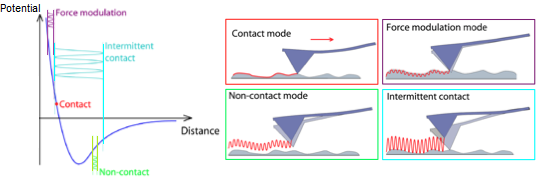
\includegraphics[width=0.5\textwidth]{AFM-fig3.png}
	\caption{Potential der Probe für eine Spitze in Funktion des Abstands. \cite{lit:grenoble} bzw. \cite{lit:jpk}}
	\label{fig:Potential}
\end{figure}

%%%%%%%%%%%%%%%%%%%%%%%%%%%%%%%%%%%%%%%%%%%%%%%%%%%%
% Abbildung mit ``Force'' betitelt, im Text als Potential verwendet - korrigieren!
%%%%%%%%%%%%%%%%%%%%%%%%%%%%%%%%%%%%%%%%%%%%%%%%%%%%





\subsection{Kraft-Distanz-Kurve}
Wie unterscheiden sich allerdings die Ergebnisse von Messungen mit verschiedenen Modi? Dies wird am besten klar, wenn man die schematische Kraft-Distanz-Kurve in Abbildung \ref{fig:Fz} betrachtet. 

\begin{figure}[h]
	\centering
	\includegraphics[width=0.5\textwidth]{}
	\caption{Kraft-Distanz-Kurve}
	\label{fig:Fz}
\end{figure}






%% TODO: Rohrscanner, Regelkreis, I-Gain & P-Gain, Wasser, Forward/Backward Scan, 



\begin{figure}[h]
	\centering
	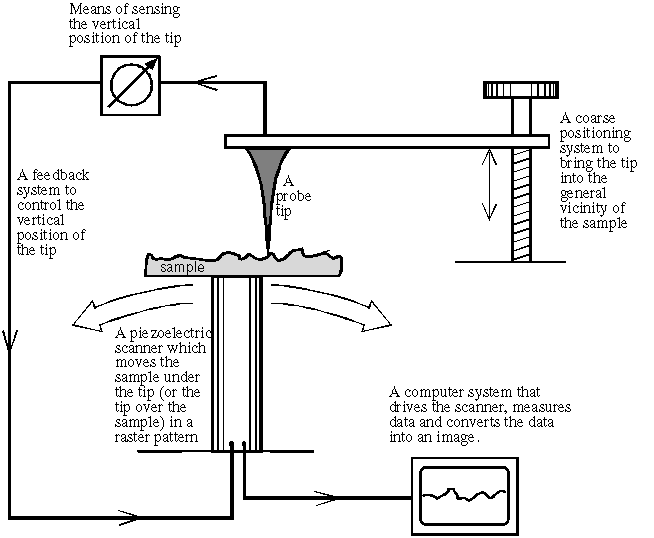
\includegraphics[width=0.5\textwidth]{regelkreis.png}
	\caption{Schematischer Aufbau des Regelkreises eines Rasterkraftmikroskops.}
	\label{fig:feedback}
\end{figure}

\subsection{}